\documentclass[docker-slim-report.tex]{subfiles}
\begin{document}

\begin{figure}[h]
    \begin{center}
        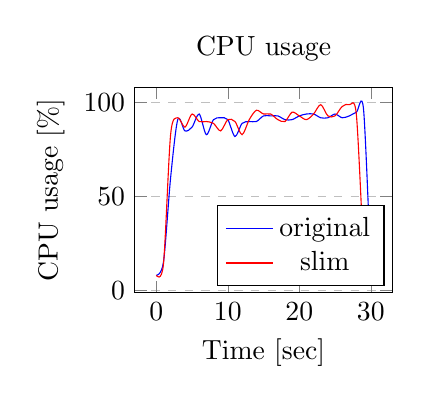
\begin{tikzpicture}
            \begin{axis}[
                smooth,
                width=0.4*\textwidth,
                title={CPU usage},
                xlabel={Time [sec]},
                ylabel={CPU usage [\%]},
                legend pos=south east,
                ymajorgrids=true,
                grid style=dashed,
            ]
                \addplot[
                    color=blue
                    ]
                coordinates {
                     (0 , 8.0) (1 , 15.0) (2 , 60.0) (3 , 91.0) (4 , 85.0) (5 , 87.0) (6 , 94.0) (7 , 83.0) (8 , 91.0) (9 , 92.0) (10 , 91.0) (11 , 82.0) (12 , 89.0) (13 , 90.0) (14 , 90.0) (15 , 93.0) (16 , 93.0) (17 , 93.0) (18 , 91.0) (19 , 91.0) (20 , 93.0) (21 , 94.0) (22 , 94.0) (23 , 92.0) (24 , 92.0) (25 , 94.0) (26 , 92.0) (27 , 93.0) (28 , 95.0) (29 , 96.0) (30 , 11.0)

                };
                \addlegendentry{original}
                \addplot[
                    color=red
                    ]
                coordinates {
                     (0 , 8.0) (1 , 14.0) (2 , 83.0) (3 , 92.0) (4 , 87.0) (5 , 94.0) (6 , 90.0) (7 , 90.0) (8 , 89.0) (9 , 85.0) (10 , 91.0) (11 , 90.0) (12 , 83.0) (13 , 91.0) (14 , 96.0) (15 , 94.0) (16 , 94.0) (17 , 91.0) (18 , 90.0) (19 , 95.0) (20 , 93.0) (21 , 91.0) (22 , 94.0) (23 , 99.0) (24 , 93.0) (25 , 93.0) (26 , 98.0) (27 , 99.0) (28 , 93.0) (29 , 17.0)

                };
                \addlegendentry{slim}
            \end{axis}
        \end{tikzpicture}
        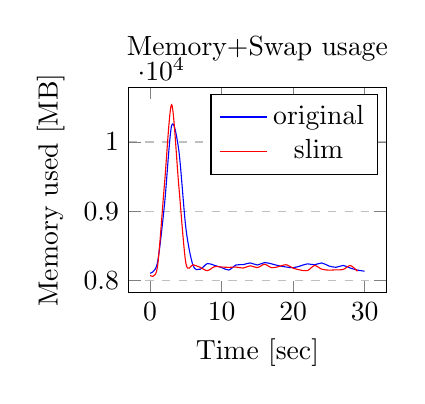
\begin{tikzpicture}
            \begin{axis}[
                smooth,
                width=0.4*\textwidth,
                title={Memory+Swap usage},
                xlabel={Time [sec]},
                ylabel={Memory used [MB]},
                legend pos=north east,
                ymajorgrids=true,
                grid style=dashed,
            ]
                \addplot[
                    color=blue
                    ]
                coordinates {
                     (0 , 8109.0) (1 , 8250.0) (2 , 9092.0) (3 , 10235.0) (4 , 9885.0) (5 , 8755.0) (6 , 8218.0) (7 , 8166.0) (8 , 8247.0) (9 , 8221.0) (10 , 8189.0) (11 , 8154.0) (12 , 8226.0) (13 , 8231.0) (14 , 8256.0) (15 , 8226.0) (16 , 8261.0) (17 , 8242.0) (18 , 8215.0) (19 , 8198.0) (20 , 8187.0) (21 , 8212.0) (22 , 8243.0) (23 , 8229.0) (24 , 8256.0) (25 , 8212.0) (26 , 8193.0) (27 , 8220.0) (28 , 8182.0) (29 , 8153.0) (30 , 8137.0)

                };
                \addlegendentry{original}
                \addplot[
                    color=red
                    ]
                coordinates {
                     (0 , 8077.0) (1 , 8186.0) (2 , 9391.0) (3 , 10539.0) (4 , 9376.0) (5 , 8250.0) (6 , 8230.0) (7 , 8193.0) (8 , 8145.0) (9 , 8202.0) (10 , 8197.0) (11 , 8192.0) (12 , 8197.0) (13 , 8182.0) (14 , 8215.0) (15 , 8188.0) (16 , 8237.0) (17 , 8187.0) (18 , 8204.0) (19 , 8231.0) (20 , 8181.0) (21 , 8154.0) (22 , 8145.0) (23 , 8219.0) (24 , 8166.0) (25 , 8152.0) (26 , 8157.0) (27 , 8161.0) (28 , 8219.0) (29 , 8136.0)

                };
                \addlegendentry{slim}
            \end{axis}
        \end{tikzpicture}
    \end{center}
    \caption{System CPU and memory usage for nginx}
\end{figure}

\end{document}
